\subsection{Stage 1: Configuration Generation}
\label{sec:stage1}

The configuration generator produces randomized alloy compositions over the
twelve elements covered by at least one of the available MEAM library files:
Al, Co, Cr, Cu, Fe, Mg, Mn, Mo, Ni, Si, Ti, and Zn. Each configuration is a
JSON object holding the species composition (mass fractions that sum to unity
at $10^{-4}$ precision), the simulation box edge in metres, the target
temperature, and the requested number of MD steps. A representative example:

\begin{verbatim}
{
  "composition": { "Al": 0.91, "Mg": 0.029, "Zn": 0.061 },
  "box_size_m": 4e-09,
  "temperature": 0.1,
  "total_steps": 1000
}
\end{verbatim}

To push the dataset towards practically interesting alloys, aluminium is
forced to be the majority species whenever it appears in a draw. Roughly
$7900$ configuration records were generated, of which $7815$ survive the
Stage~2 physicality filter described in Section~\ref{sec:stage2}. That
surviving set is the corpus quoted throughout this report. The
element-occurrence counts are shown in Figure~\ref{fig:element_freq}:
aluminium appears in about $45\,\%$ of records, consistent with the
dominance rule, while every other element is sampled in roughly $30$ to
$37\,\%$ of records. That coverage gives the Stage~4 merge logic enough
data to seed each binary interaction.

\begin{figure}[htbp]
	\centering
	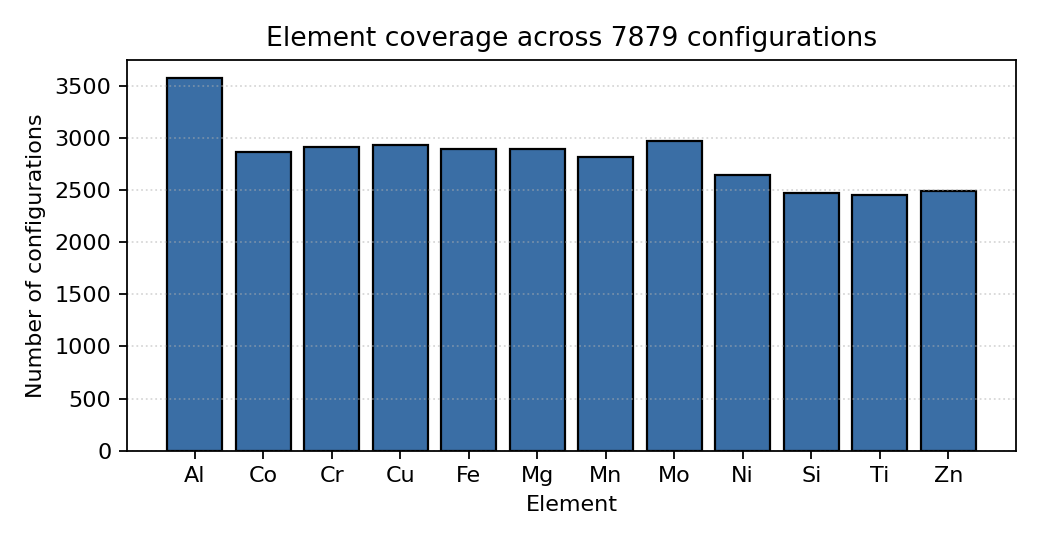
\includegraphics[width=0.85\textwidth]{figures/element_frequency.png}
	\caption{Number of configurations in which each element is present, over
	the retained corpus. The dominance of Al reflects the bias rule that keeps
	aluminium as the majority species whenever it is drawn.}
	\label{fig:element_freq}
\end{figure}
